% ==========================================================================================================================
\section{Modelo de administración de red de SNMP}
% ==========================================================================================================================

\noindent
A continuación se muestran se muestran los resultados de la herramienta creada por medio de las siguientes operaciones.

\noindent
\newline
\textbf{Operación 1:} Se agrega un agente LINUX con el nombre ''comunidadEquipo3grupo4CM1''. Haciendo una consulta SNMP con la comunidad dada de alta obtenemos la información de ésta misma, como se muestra en la imagen debajo.  
 
\begin{figure}[htbp!]
	\centering
		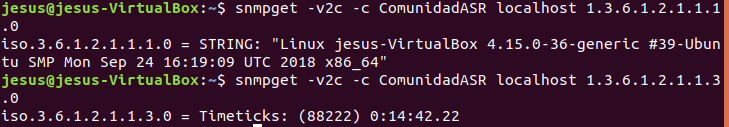
\includegraphics[width=0.8\textwidth]{images/tarea3/op1}
	\caption{Operación 1a.}
\end{figure}